\chapter{目标代码优化}

\label{chap:optimize}
在上一章中,我们生成了一串可执行的 asm 指令,但 CPU 在实际运行它时,所执行的指令数量较大,从而导致执行性能变差。
本章我们将通过一些操作来减少 CPU 实际运行时所执行的指令数量,从而提高程序的执行效率。

\begin{remark}
本章的参考资料有:
\begin{itemize}
    \item 现代编译原理:C 语言描述\cite{TigerBook}
    \item 编译原理\cite{DragonBook}
    \item \textit{Engineering a Compiler}\cite{EngineeringACompiler}
    \item SSA Construction \& Destruction\cite{SSAConstructionAndDestruction}
\end{itemize}
\end{remark}

\section{什么是优化?}

比较以下两串等价的 asm 代码:
\begin{lstlisting}
    addi rd, rs1, 1
    addi rd, rs1, 2
\end{lstlisting}
\begin{lstlisting}  
    addi rd, rs1, 3
\end{lstlisting}

两串代码实现了同样的功能。第一串代码使用了2条指令,第二串代码只用了1条指令。
我们的「优化」指的就是在不影响运行结果(输出)的前提下,尽可能把指令数量减少。
例如像上文中把第一串代码优化成第二串代码的过程,就是一种优化。

当然,存在非常简单的优化,例如你可以把诸如 \texttt{addi x0, x0, 0} 这样的指令删除,
但这样的优化,在效果上的泛化性是不够的。
本章节将为大家介绍一些更加复杂的优化方法,如寄存器分配、Mem2Reg 等。

\section{基本块划分}

我们日常写的程序通常有着较为复杂的逻辑,包括分支、循环等结构。
如果我们以一条指令为单位,控制流将变得非常复杂,因此我们提出\textbf{基本块 (Basic Block)} 的概念。
一个基本块由前驱、后继和一串顺序执行的指令(即这串指令中不存在任何跳转指令)组成。
所有的跳转逻辑,通过维护基本块之间的前驱、后继关系来保证。
通过基本块的划分,目标程序自然地被表示成一张有向图,图的节点就是这些基本块,边表示了他们之间的跳转关系。
上面提到的由以基本块为节点的有向图,被称作\textbf{控制流图 (Control Flow Graph, CFG)}。
下面提到的活跃分析,将在控制流图的基础上进行。

\section{活跃分析}

活跃分析可以告诉我们一个函数中的变量在程序执行过程中是否处于活跃状态。
处于活跃状态的变量在程序执行过程中,其值可能被使用。反之,不活跃的变量在程序执行过程中,其值不会被使用。

粗略地,我们有这样的想法:在同一时间戳活跃的变量不应该占用同一个寄存器,否则会导致数据冲突。
就此我们能够构建出冲突图,从而进行寄存器分配。这个我们留到后面讲。

\subsection{概念}

以下是活跃分析中的一些概念定义:

\begin{description}
    \item[def 和 use:]def 是在一条指令中被赋值,即被定义的变量;use 指在这条指令中被使用的变量。
例如:在以下语句中,\texttt{a} 是 def,\texttt{b} 和 \texttt{c} 是 use。
\begin{lstlisting}[language=c]
    a = b + c
\end{lstlisting}

首先为了简单起见,我们先假设每个基本块只包含一条指令。后面我们会介绍包含多条指令的基本块的等效 use 和 def。

\item[活跃:] 表示这个变量的值将来还要继续使用。一个变量在一条边上活跃,
  指存在一条从这条边通向它的一个 use 且不经过任何它的 def 的有向路径(即保持当前的值直到被下一次使用)。

\item[入口活跃:] 一个变量在一个块中是入口活跃的,当且仅当这个变量在当前块节点存在一条入边是活跃的。
  注意,根据活跃的定义,这等价于这个变量在当前块节点的所有入边都是活跃的。

\item[出口活跃:] 一个变量在一个块中是出口活跃的,当且仅当这个变量在当前块节点存在一条出边是活跃的。

\end{description}

\subsection{活跃分析的算法}

变量(当然你可以称之为虚拟寄存器)在每个块中的活跃状态可由它们的 def 和 use 算出。对每个节点 $n$ 都有:
(下文中 $\mathit{suc}$ 表示后继节点的集合)
\begin{align}
\label{live-analysis-data-flow-1}\mathit{in}[n]  &= \mathit{use}[n] \cup (\mathit{out}[n] - \mathit{def}[n]), \\
\label{live-analysis-data-flow-2}\mathit{out}[n] &= \bigcup_{s \in \mathit{suc}[n]} \mathit{in}[s].
\end{align}
以及边界条件:
\begin{align}
\label{live-analysis-data-flow-3}\mathit{out}[\mathit{exit}] = \emptyset
\end{align}
上面的式子被称为\textbf{活跃分析的数据流方程}。

\begin{itemize}

\item 对于 $\mathit{out}[n]$ 中的变量,如果它在这个块中没有被 def 过,则它一定在 $\mathit{in}[n]$ 中。这一点是符合直觉的。因为,一个变量出口活跃,那么说明这个变量将会在之后的语句中被use。那么,这个值一定要在先前被def过,并且一路传递到了use处。是故,只有两种可能:要么在当前块被def,要么是从之前的块中传入的。

\item $\mathit{use}[n]$ 一定都属于 $\mathit{in}[n]$,因为use的值不可能在语句自身处被定义,所以一定是从其他语句处传入的。

\item 是故,综合上述两部分,我们可以得到$\mathit{in}[n]$ 的构成:当前块中使用的变量,即 $\mathit{use}[n]$;以及之后块中需要使用的变量,但是并未在该块中定义的变量,即 $\mathit{out}[n] - \mathit{def}[n]$。

\item 如果一个变量在当前块的某个后继中是入口活跃的,则它在当前块中一定是出口活跃的。
因为它在当前块的该后继的所有入边都活跃,则在当前块连着这个后继的那条边上,它一定是活跃的。

\item 边界条件:所有变量在函数结束时都消亡了。
\end{itemize}

具体地,我们的算法可以通过不动点迭代的方式进行。一般来说,是从出口开始倒序地 BFS 遍历控制流图,
因为出口处的边界条件是确定的。
对所有的基本块都可以进行如上的迭代,直到收敛(一次完整迭代前后没有变动)为止。

\subsection{基本块的等效 use/def}

前面假设了一个基本块只包含一条指令。现在我们从活跃分析的流方程出发,来推导包含多条指令的基本块的等效 use/def。

包含多条指令的基本块可以视为由两个更小的基本块合并而成。
因此,我们只考虑两个由两条语句组成的基本块。设这两条语句为 $p$, $n$,基本块为 $pn$。
由基本块的性质。每个基本块只有一个入口。因此基本块的入口活跃变量等价于这个基本块中,第一条语句的入口活跃变量。
进而有:
\begin{align*}
  \mathit{in}[pn] &= \mathit{in}[p] = \mathit{use}[p] \cup (\mathit{out}[p] - \mathit{def}[p]) \\
\end{align*}
同时,由基本块的性质 $\mathit{out}[p] = \mathit{in}[n]$。这是显然的,因为基本块内,没有其他的控制流转换,所以前一条语句的出口活跃变量,一定是后一条语句的入口活跃变量。进而:
\begin{align*}
  &= \mathit{use}[p] \cup (\mathit{in}[n] - \mathit{def}[p]) \\
\end{align*}
根据式(4.1)进行展开,可以得到:
\begin{align*}
  &= \mathit{use}[p] \cup \left(\mathit{use}[n] \cup (\mathit{out}[n] - \mathit{def}[n]) - \mathit{def}[p]\right) \\
\end{align*}
由集合的性质,可以得到:
\begin{align*}
  &= \mathit{use}[p] \cup (\mathit{use}[n] - \mathit{def}[p]) \cup (\mathit{out}[n] - \mathit{def}[n] - \mathit{def}[p]) \\
\end{align*}
由并集的结合律,我们可以给它加上一个美观的括号,更加贴近我们在式(4.1)中的形式。
\begin{align*}
  &= \left(\mathit{use}[p] \cup (\mathit{use}[n] - \mathit{def}[p])\right) \cup \left(\mathit{out}[pn]
   - (\mathit{def}[n] \cup \mathit{def}[p])\right).
\end{align*}

所以我们可以把 $\mathit{use}[p] \cup (\mathit{use}[n] - \mathit{def}[p])$ 视为 $pn$ 的等效 use,
把 $\mathit{def}[n] \cup \mathit{def}[p]$ 视为 $pn$ 的等效 def。从直觉上去考虑这件事情,这是很正确的。一个块的等效def当然等价于每一条语句def的并集喽!等效use,则应当是那些在块中使用的变量,却没有在该基本块中,在使用该变量之前的前驱语句中定义的变量。因为从宏观上去看,剩下的那些use变量,在块内自我消化掉了,不用再依靠其他的块来输入这个变量。

因此,我们可以首先计算出每个基本块的等效use和等效def。然后,以函数出口的活跃变量集合为空集为初始迭代条件,将这些块压入一个队列中,依次处理队头的基本块。在处理过程中,我们先暂时假定出口活跃的变量是“正确的”,然后据此根据式(4.1),计算该基本块的入口活跃变量。随后,根据式(4.2),更新CTG中该基本块所有的前驱块的出口活跃变量,并将那些确实得到更新的基本块也加入队列中,重复上述操作,直至所有基本块的出口、入口变量皆不再更新。

这样,我们就获得了每个基本块的出口活跃变量和入口活跃变量。在实际操作过程中,我们可以只利用出口活跃变量,对基本块中的语句进行倒序遍历。由于基本块只有一个出口,所以一个基本块的出口活跃变量,即为该基本块中最后一句语句的出口活跃变量,可以此为基本块之初始条件。此外,计算每一句语句的use和def是平凡的。是故,我们可以根据每一句语句的出口活跃变量,计算出其入口活跃变量。由基本块的性质,该语句的入口活跃变量,即为基本块中该语句的前驱的出口活跃变量。重复此类操作,我们就可以得到每一条语句处的出口、入口活跃变量。

\section{Mem2Reg 优化}\label{mem2reg}

在从抽象语法树到 LLVM IR 的转换时,我们使用 \texttt{alloca} 指令来处理局部变量
(\ref{AST-to-IR-local-variables})。尽管这样处理起来十分方便,然而每次使用都需要读写内存,
效率不高,因此 LLVM 提供了一个将 \texttt{alloca} 指令转化为虚拟寄存器的方案来提升效率。
此外,这样的操作也会方便静态分析,因为相较于虚拟寄存器,内存的数据更难分析。这个优化被称为 Mem2reg,
Mem 是指 \texttt{alloca} 指令将数据存于内存中,Reg 是指优化后数据将会放在虚拟寄存器中,
整个优化的过程即为将通过 \texttt{alloca} 指令而存在内存中数据迁移到寄存器中,因而称作 Mem2Reg。

在 Mem2Reg 优化的过程中,我们的目标是尽可能减少 \texttt{alloca} 的数量。具体的优化方法有(注意下文中的 def 和
use 是指 \texttt{alloca} 产生的空间的 def 和 use)
\begin{enumerate}
    \item 没有被使用的 \texttt{alloca} 可以直接去掉;
    \item 如果只被定义了一次,那么所有的使用都可以用定义的值代替;
    \item 如果一个 \texttt{alloca} 的定义使用只出现在一个块中,那么每个 use 可以被最近的 def 替换;
    \item 如果一个 \texttt{alloca} 只被 \texttt{load} 和 \texttt{store},那么可以通过在支配边界插入
        \texttt{phi} 指令,并将所有的 use 替换为对应的 \texttt{phi} 指令的结果。
\end{enumerate}
经过上述的优化方法,大多数 \texttt{alloca} 指令都可以被去掉。前 3 个方法较为简单,本文不会详细介绍;
第 4 个方法将会在后文中详细介绍。

由于 Mx* 语言没有取地址之类的指令,所以所有的 \texttt{alloca} 指令理论上都可以被消除。

\subsection{静态单赋值形式 (SSA) 与 \texttt{phi} 指令}

在编译器中,静态是指不运行程序,与动态相对。静态单赋值形式 (Static Single Assignment),
即静态来看每个变量只被赋值一次,也就是函数中只有一个对其赋值的指令。这里需要注意,即便符合 SSA 形式,
如果多次执行赋值指令所在的块,这个变量也会被多次赋值。

在我们的LLVM程序中,可能会出些一些\texttt{alloca}指令。\texttt{alloca}出的指针\textbf{仅被赋值一次}。但是,\texttt{alloca}出的指针指向的内容,是可以被赋值多次的。在下文中,我们把这个\texttt{alloca}出的指针简称作\texttt{ptr},\texttt{*ptr}表示其指向的内容。

所以,\texttt{alloca}指令的存在,是为了降低我们的心智压力,使得\texttt{*ptr},可以根据我们的需要不断修改,从而达到一般程序中变量的效果。但是,这样做的坏处也显而易见:我们需要不断地到栈空间去读取和修改,降低了程序的效率,因此,我们可以发扬人类的智慧,想办法确定在不同的语句中,\texttt{*ptr}到底是多少。

平凡地,如果我们的程序是完全顺序执行的,那么我们不难想到,可以用一个map去维护不同的\textbf{alloca出的指针}的当前值。每产生一次\texttt{store}指令,就去更新对应的\texttt{*ptr}。遇到所有的\texttt{load}指令,我们可以直接删除。比如如下指令:

\begin{lstlisting}[language=LLVM]
    %ptr = alloca i32
    %init = add i32, 114, 514
    store i32 %init, ptr %ptr
    %x = load i32, ptr %ptr
    %y = add i32, 1, %x
\end{lstlisting}

我们可以简单地改写成:

\begin{lstlisting}[language=LLVM]
    %init = add i32, 114, 514
    %y = add i32, 1, %init
\end{lstlisting}

但是,棘手的地方在于,我们的程序并不是完全的顺序结构,我们会遇到分支结构和循环结构。在此等状况下,我们很有可能会遇到在不同的分支上,某个\texttt{*ptr}截然不同的情况。请看下面的例子:

\begin{lstlisting}[language=C]
// 这是一段简单的 C 代码
int main() {
    int x = 2, y = 3;
    int b;
    if(x + 1 > y) {
        b = -1;
        //branch 1
    } else {
        b = 1;
        //branch 2
    }
    //merge
    return b;
}
\end{lstlisting}

显而易见,在branch1和branch2中的b的值是截然不同的。按照我们的老方法,非常朴素地,会得到这样的IR:

\begin{lstlisting}[language=LLVM]
; 不带优化的 LLVM IR
define i32 @main() {
entry:
  %retval = alloca i32, align 4
  %x = alloca i32, align 4
  %y = alloca i32, align 4
  %b = alloca i32, align 4
  store i32 0, i32* %retval, align 4
  store i32 2, i32* %x, align 4
  store i32 3, i32* %y, align 4
  %0 = load i32, i32* %x, align 4
  %add = add nsw i32 %0, 1
  %1 = load i32, i32* %y, align 4
  %cmp = icmp sgt i32 %add, %1
  br i1 %cmp, label %if.then, label %if.else

if.then:                                          ; preds = %entry
  store i32 -1, i32* %b, align 4
  br label %if.end

if.else:                                          ; preds = %entry
  store i32 1, i32* %b, align 4
  br label %if.end

if.end:                                           ; preds = %if.else, %if.then
  %2 = load i32, i32* %b, align 4
  ret i32 %2
}
\end{lstlisting}

但是,这值得吗?这个程序,我们简单地分析下,就可以得到在branch1中b为-1,在branch2中b为1。我们应当有一些方法,去告知我们的程序:“当控制流是从branch1来到merge时,b应该是1;控制流从branch2来到merge时,b应当是-1。”

这个时候,我们就可以使用\texttt{phi}指令来解决这个问题了。\texttt{phi}指令的一般形式如下:

\begin{lstlisting}[language=LLVM]
    %obj = phi <type> [ <val1>, <block1> ], [ <val2>, <block2> ], [ <val3>, <block3> ]
\end{lstlisting}

每一个中括号中包含一个value-block对。这条\texttt{phi}指令的含义是,当控制流从第i个block跳来时,obj的值应当是第i个value。运用上\texttt{phi}指令进行mem2reg优化,我们就可以得到这样的IR:

\begin{lstlisting}[language=LLVM]
; 带 Mem2Reg 优化的 LLVM IR
define i32 @main() {
entry:
  %add = add nsw i32 2, 1
  %cmp = icmp sgt i32 %add, 3
  br i1 %cmp, label %if.then, label %if.else

if.then:                                          ; preds = %entry
  br label %if.end

if.else:                                          ; preds = %entry
  br label %if.end
    
if.end:                                           ; preds = %if.else, %if.then
  %b.0 = phi i32 [ -1, %if.then ], [ 1, %if.else ]
  ret i32 %b.0
}
\end{lstlisting}

经过这样的优化,我们成功地移除了\texttt{alloca}指令,并且没有对程序的效果产生影响。但是代码干净了许多,性能也提升了不少。那么,我们不得不开始思考一个问题,我们到底应该怎么做呢?

很显然,mem2reg优化首先需要我们构建正确的控制流图。然后,我们需要考虑,应当给哪些变量,在哪里放置\texttt{phi}。最后,我们需要给每个\texttt{phi}指令添上正确的block-value对,并且移除\texttt{alloca}及与\texttt{alloca}相关的冗余指令。

构建控制流图在活跃分析部分已经阐述,故于此不复赘述。现在,我们首先要解决的问题,就是应该给哪些变量,在哪里放置\texttt{phi}指令。因此,我们需要引入\textbf{必经节点}的概念。

\subsection{支配关系的确定}

首先,我们先引入一些必要的概念:

\begin{description}
    \item[必经节点 (Dominate)]
    如果每一条从流图的入口节点到节点 $n$ 的路径都经过节点 $d$, 我们就说 $d$ 是 $n$ 的必经节点,记为 $d$ dom $n$。
    请注意,在这个定义下每个节点都是自己的必经节点。

    \item[严格必经节点 (Strictly Dominate)]
    $d$ 是 $n$ 的严格必经节点,当且仅当 $d$ 是 $n$ 的必经节点 且 $n\neq d$, 记作 $d$ sdom $n$。

    \item[支配集]
    节点 $n$ 的支配集是所有 $n$ 的必经节点的集合,记为 $\mathit{Dom}(n)$。

    \item[最近必经节点 (Immediate Dominator, IDom)]
    在支配集中,我们把从流图入口到节点 $n$ 所经过的路径上,最后一个 $n$的严格必经节点,称为$n$的最近必经节点。

    \item[支配树 (Dominator Tree)]
    通过节点之间的必经节点关系,我们就可以依此来建立一颗支配树。在支配树中,节点 a 是 b 的父亲,当且仅当 a 是 b 的最近必经节点。

    \item[支配边界 (Dominance Frontier)]
    Y 是 X 的支配边界,当且仅当 X 是 Y 的一个前驱节点(在 CFG 中)P 的必经节点,并且 X 并不是 Y 的严格必经节点。请看下图之例。比如,B 是 E 的前驱节点,同时 B 是 B 的必经节点,并且 B 不是 E 的严格必经节点。因此,E 是 B 的支配边界。从直觉上去考察这件事,支配边界实质上在表征到达这个点后,数据流可能会发生和其他数据流合并的情况。
    \begin{figure}[h]
        \centering
        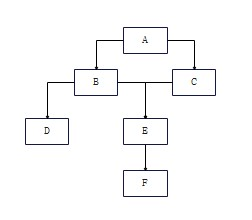
\includegraphics[width=0.5\linewidth]{CTG.jpg}
        \caption{控制流图}
        \label{fig:enter-label}
    \end{figure}
\end{description}

\subsubsection{确定支配集}

首先我们有:$\mathit{Dom}(n) = \{n\} \bigcup \left(\bigcap_{m\in \mathit{preds}(n)} \mathit{Dom}(m)\right)$。
即:一个节点的支配集等于其所有前驱节点(ctg)支配集的交集再并上自身。
这是显而易见的。根据支配集的定义,即所有必经节点的集合。根据定义,每个节点一定是自己的必经节点。所有前驱节点支配集的交集,即在表征所有前驱节点中共有的那些必经节点。因此,这两部分的并集就是这个节点的所有必经节点集合,也就是这个节点的支配集了。

我们可以通过对每个节点的迭代来计算支配集,即先假设所有节点的支配集都是节点全集,
并保证入口块没有入度(绝大多数情况下,入口块一定都没有入度),然后不断迭代直到收敛。
具体地,你可以在迭代的每一步都运行一遍 $\mathit{Dom}(n) \leftarrow \{n\} \bigcup
\left(\bigcap_{m\in \mathit{preds}(n)} \mathit{Dom}(m)\right)$,
直到一遍下来所有 $\mathit{Dom}(n)$ 不发生变化为止。
由于控制流图是前向传播的,所以这里迭代的顺序一般采用 BFS 序。

这样我们就获得了所有的 $\mathit{Dom}(n)$, 也就是获得了所有节点的支配关系。

\subsubsection{确定最近必经节点 (IDom)}

我们观察到支配集具有一个重要性质——节点 n 的支配集里任意两个不同的节点中,一个节点 A 必然是另一个节点 B 的必经节点。若非如此,就会存在只经过其中一个节点,就到达节点 n 的路径,这和支配集的性质相矛盾。因此,我们可以发现,每个节点支配集中的所有元素构成一条链,且直接支配节点的支配集元素比当前节点少1(实际上,如果按照这些元素的支配集元素个数排序,这些元素的支配集元素每个之间都差 1)。
因此,要确定当前节点的直接支配节点,只需要找到支配集元素个数为当前节点的支配集元素个数减 1 的节点。
注意,同样因为刚才的性质,这样的节点数量有且只有一个。

\subsubsection{支配树构建算法}

根据每个节点的直接支配节点,我们可以建构支配树。每个节点的直接支配节点到对应节点连边。
由于除入口节点外的每个节点入度都为 1,这样的图构成一棵支配树。

\subsubsection{确定支配边界}

根据支配边界的定义,一个节点 X 是节点 Y 的支配边界,当且仅当 Y 在 X 的一个控制流前驱节点的支配集中但 Y 不在 X 的支配集中。
因此,$n$ 是且仅是 $\bigcup_{m\in\mathit{preds}(n)}\left(\mathit{Dom}(m)-(\mathit{Dom}(n)-\{n\})\right)$
中元素的支配边界。

基于上面的原理,通过遍历所有基本块,我们就可以确定所有基本块的支配边界了。

\subsubsection{求支配集的其他方法}

以上的方法是通过迭代的方式求解支配集的。在控制流图节点数量较少的情况下,其时间复杂度是可以接受的。
然而,在某些极端的情况下,这种方法的时间复杂度是 $O(n^2)$ 的,可能会导致性能问题。以下给出两个求支配集的更高效的方法:

1. bitset 优化集合操作:注意到在迭代过程中,我们只需要对支配集进行交集、并集等操作,因此可以使用 bitset 位运算来加速这些操作。
2. Lengauer-Tarjan 算法:该算法可以在接近线性的时间复杂度内求解支配集。

以上两种做法,均在 OI-wiki \url{https://oi-wiki.org/graph/dominator-tree/} 中有详细介绍,感兴趣的读者可以参考。

\subsection{\texttt{phi} 指令放置算法}

\texttt{phi} 指令的放置分为两个步骤——预留 \texttt{phi} 指令和替换原来的变量使用。

对于加入 \texttt{phi} 指令,我们需要先收集所有被定义过的变量名(即 \texttt{alloca} 指令的结果),
再对每个变量名遍历找到所有变量的 def,在这些 def 所在块的支配边界的头部预留 \texttt{phi} 指令。
然后对预留了 \texttt{phi} 指令的块的支配边界头部再预留 \texttt{phi} 指令。重复操作,
直到没有新的支配边界或者对应块的支配边界已经预留了对应变量的 \texttt{phi} 指令。

\texttt{phi} 指令放置完毕后,我们需要对变量的使用进行重命名,即维护好之前提到的变量的 “版本”。
重命名的过程包括:为所有的 use 替换变量名、确定 \texttt{phi} 指令中不同块进入对应的值。一种可行的方式是为每个变量名开一个栈。这一步骤,我们可以在支配树上完成。具体的操作为
\begin{itemize}
  \item 在每个基本块中,首先应当对入口顶部的 \texttt{phi} 指令进行处理。我们要为这些\texttt{phi} 指令指定一个合适的\texttt{obj}名。然后,我们需要把这个\texttt{obj}名,压入这条\texttt{phi} 指令对应的 \texttt{alloca} 指令对应变量的对应栈中。对于每一个\texttt{alloca}指令对应的变量,我们都应该创建一个栈。栈顶就是当前的变量值。
  \item 在基本块中所有的操作都已经重写之后,我们将使用当前的形式名重写程序块在 CFG 中各后继节点中的适当 \texttt{phi} 指令的参数,即用当前对应栈的栈顶元素更新之。
  \item 最后,对当前基本块在支配树中的子节点进行递归处理,这是一个在支配树上 DFS 的过程。
  \item 当算法从一个基本块返回时,应当弹出所有的,在本基本块中压入的元素都应当被弹出。将所有的栈恢复原状。
\end{itemize}

请看下面的例子:

\begin{lstlisting}[language=LLVM]
define i32 @main() {
entry:
  %retval = alloca i32, align 4
  %x = alloca i32, align 4
  %y = alloca i32, align 4
  %b = alloca i32, align 4
  store i32 0, i32* %retval, align 4
  store i32 2, i32* %x, align 4
  store i32 3, i32* %y, align 4
  %0 = load i32, i32* %x, align 4
  %add = add nsw i32 %0, 1
  %1 = load i32, i32* %y, align 4
  %cmp = icmp sgt i32 %add, %1
  br i1 %cmp, label %if.then, label %if.else

if.then:                                          ; preds = %entry
  store i32 -1, i32* %b, align 4
  br label %if.end

if.else:                                          ; preds = %entry
  store i32 1, i32* %b, align 4
  br label %if.end

if.end:                                           ; preds = %if.else, %if.then
  %2 = load i32, i32* %b, align 4
  ret i32 %2
}
\end{lstlisting}

这个程序的支配树非常简单,即entry为根节点,剩余三个块均为entry的子节点。
经过\texttt{phi} 指令放置算法后, 我们的if.end块会变成这样:

\begin{lstlisting}[language=LLVM]
if.end:
  %b = phi i32 [ , %if.then ], [ , %if.else ]
  %2 = load i32, i32* %b, align 4
  ret i32 %2
\end{lstlisting}

为了方便演示,我们令这三个子节点的访问顺序是if.then, if.end, in.else.在访问完if.then块后,if.end块会变成:

\begin{lstlisting}[language=LLVM]
if.end:
  %b = phi i32 [ -1, %if.then ], [ , %if.else ]
  %2 = load i32, i32* %b, align 4
  ret i32 %2
\end{lstlisting}

在访问if.end块过程中,首先,重写\texttt{phi} 指令:

\begin{lstlisting}[language=LLVM]
; 不带优化的 LLVM IR
if.end:
  %phi = phi i32 [ -1, %if.then ], [ , %if.else ]
  %2 = load i32, i32* %b, align 4
  ret i32 %2
\end{lstlisting}

我们将\texttt{\%phi}这个名字压入\%b对应的栈中。 

检查该基本块,我们发现存在一条对\%b的\texttt{load} 指令。由于SSA的特性,Load的结果,即\%2的值从此被固定下来了。此时,\%b对应的栈,栈顶元素是\text{\%phi},我们可以另外在开一个map,存储\%2中的值是多少。经过改写,我们得到:

\begin{lstlisting}[language=LLVM]
if.end:
  %phi = phi i32 [ -1, %if.then ], [ , %if.else ]
  ret i32 %phi
\end{lstlisting}

然后,我们退出if.end块,同时将\%phi弹出。最后,我们访问if.else块,更新\texttt{phi}指令的值:

\begin{lstlisting}[language=LLVM]
if.end:
  %phi = phi i32 [ -1, %if.then ], [1, %if.else ]
  ret i32 %phi
\end{lstlisting}

大功告成!接下来要做的,就是诸如删除alloca指令之类的操作,这是很平凡的工作了。

\subsection{静态单赋值形式 (SSA) 的消除} \label{SSA-eliminate-phi}

经过 Mem2Reg,我们生成了很多 \texttt{phi}。然而,汇编中没有 \texttt{phi} 指令的直接对应,所以我们须将其消除,
用等价的其余指令如 \texttt{move} 来代替(注意这里的 \texttt{move} 属于内部实现,既不是 LLVM IR 的指令,
也不属于汇编)。一般地,我们在拥有 \texttt{phi} 指令的这个块的前驱块中插入一份拷贝,
例如图 \ref{fig:SSA-eliminate-phi-1}(BB 表示 \textbf{B}asic \textbf{B}lock)。

\begin{figure}[htb]
\centering
\begin{tikzpicture}[
squarednode/.style={rectangle, draw=black!100, fill=black!5, very thick, minimum size=5mm, align=center},
nothing/.style={circle, draw=white, minimum size=0}
]
\node[squarednode] (BB1) {BB1\\\texttt{x1=0}};
\node[nothing] (mid) [below=of BB1] {};
\node[squarednode] (BB2) [left=of mid] {BB2\\\texttt{x2=1}};
\node[squarednode] (BB3) [right=of mid] {BB3\\\texttt{x3=2}};
\node[squarednode] (BB4) [below=of mid] {BB4\\\texttt{x4=phi [x2, BB2], [x3, BB3]}};

\draw[thick,->] (BB1) -- (BB2.north);
\draw[thick,->] (BB1) -- (BB3.north);
\draw[thick,->] (BB2.south) -- (BB4);
\draw[thick,->] (BB3.south) -- (BB4);
\end{tikzpicture}
\begin{tikzpicture}[
squarednode/.style={rectangle, draw=black!100, fill=black!5, very thick, minimum size=5mm, align=center},
nothing/.style={circle, draw=white, minimum size=0}
]
\node[nothing] (BB1) {};
\node[nothing] (mid) [below=of BB1] {};
\node[nothing] (BB2) [left=of mid] {};
\node[nothing] (BB3) [right=of mid] {};
\node[nothing] (BB4) [below=of mid] {};

\draw[very thick, draw=black!50, ->] (BB2) -- (BB3);
\end{tikzpicture}
\begin{tikzpicture}[
squarednode/.style={rectangle, draw=black!100, fill=black!5, very thick, minimum size=5mm, align=center},
nothing/.style={circle, draw=white, minimum size=0}
]
\node[squarednode] (BB1) {BB1\\\texttt{x1=0}};
\node[nothing] (mid) [below=of BB1] {};
\node[squarednode] (BB2) [left=of mid] {BB2\\\texttt{x2=1}\\\texttt{x4=x2}};
\node[squarednode] (BB3) [right=of mid] {BB3\\\texttt{x3=2}\\\texttt{x4=x3}};
\node[squarednode] (BB4) [below=of mid] {BB4};

\draw[thick,->] (BB1) -- (BB2.north);
\draw[thick,->] (BB1) -- (BB3.north);
\draw[thick,->] (BB2.south) -- (BB4);
\draw[thick,->] (BB3.south) -- (BB4);
\end{tikzpicture}
\captionsetup{justification=centering}
\caption{左图为消除 \texttt{phi} 前的控制流图,右图为 \texttt{phi} 消除后的控制流图。\\可以发现右图将 \texttt{x4} 对应的取值插入到了 BB2 和 BB3 中。}
\label{fig:SSA-eliminate-phi-1}
\end{figure}

这样的操作能解决大部分的 \texttt{phi} 指令,但是还有一些特殊情况需要处理,例如图
\ref{fig:SSA-eliminate-phi-2} 的左图。

\begin{figure}[htb]
\centering
\begin{tikzpicture}[
squarednode/.style={rectangle, draw=black!100, fill=black!5, very thick, minimum size=5mm, align=center},
nothing/.style={circle, draw=white, minimum size=0}
]
\node[squarednode] (BB1) {BB1};
\node[nothing] (mid1) [right=of BB1] {};
\node[nothing] (mid2) [below=of BB1] {};
\node[squarednode] (BB2) [left=of mid2] {BB2};
\node[squarednode] (BB3) [right=of mid2] {BB3};
\node[squarednode] (BB4) [right=of mid1] {BB4};

\draw[thick,->] (BB1) -- (BB2);
\draw[thick,->] (BB1) -- (BB3);
\draw[thick,->] (BB4.south) -- (BB3);
\end{tikzpicture}
\begin{tikzpicture}[
squarednode/.style={rectangle, draw=black!100, fill=black!5, very thick, minimum size=5mm, align=center},
nothing/.style={circle, draw=white, minimum size=0}
]
\node[nothing] (BB1) {};
\node[nothing] (mid) [below=of BB1] {};
\node[nothing] (BB2) [left=of mid] {};
\node[nothing] (BB3) [right=of mid] {};
\node[nothing] (BB4) [below=of mid] {};

\draw[very thick, draw=black!50, ->] (BB2) -- (BB3);
\end{tikzpicture}
\begin{tikzpicture}[
squarednode/.style={rectangle, draw=black!100, fill=black!5, very thick, minimum size=5mm, align=center},
nothing/.style={circle, draw=white, minimum size=0}
]
\node[squarednode] (BB1) {BB1};
\node[nothing] (mid1) [below=of BB1] {};
\node[squarednode] (BB2) [left=of mid1] {BB2};
\node[squarednode] (BB5) [right=of mid1] {BB5};
\node[nothing] (mid2) [right=of BB5] {};
\node[squarednode] (BB4) [right=of mid2] {BB4};
\node[squarednode] (BB3) [below=of mid2] {BB3};

\draw[thick,->] (BB1) -- (BB2);
\draw[thick,->] (BB1) -- (BB5);
\draw[thick,->] (BB5) -- (BB3);
\draw[thick,->] (BB4.south) -- (BB3);
\end{tikzpicture}
\captionsetup{justification=centering}
\caption{左图为原控制流图,右图为插入新基本块 BB5 后的控制流图。\\BB1 到 BB3 构成 critical edge,有数据冲突隐患,因此二者间需要插入空基本块 BB5 以消除 critical edge。}
\label{fig:SSA-eliminate-phi-2}
\end{figure}

我们看到图 \ref{fig:SSA-eliminate-phi-2} 左图的 BB1 有两个后继,BB3 有两个前驱。
假设 BB2、BB3 都有 \texttt{phi} 指令,则它们都会往 BB1 插入拷贝,这就会导致该变量在 BB1 上被修改,
从而影响到 BB2 所在的分支进而引起数据冲突。我们发现,BB1 与 BB3 之间的这条边有这样的特点:
出端有多个后继且入端有多个前驱。我们称这样的边为 \textbf{critical edge}。

所有的 critical edge 都可能会引起上述的数据冲突。
为了解决 critical edge,我们需要在 critical edge 中间插入一个新的空基本块 BB5 以消除 critical edge。
BB3 中的 \texttt{phi} 指令会往 BB5 和 BB4 中插入拷贝,而 BB2 中的 \texttt{phi} 指令会往
BB1 中插入拷贝,这样就不会有数据冲突了。

值得一提的是,在上图中,BB2 和 BB1 之间的 edge 也是 critical edge(BB2 既然有
\texttt{phi} 指令,它必定是有多个前驱的,否则这个 \texttt{phi} 指令可以直接被消除)。
为了方便展示,图里并没有画出来,实际上也需要在此插上空块。

同时,在汇编代码翻译的过程中,我们也需要注意数据冲突发生的可能性。比如说,我们可能在翻译过程中,产生这样的语句:
\begin{lstlisting}
	mv	a2, a0
	mv	a1, a2
 	mv	a0, a1
\end{lstlisting}

经过如上精彩绝伦的操作,我们成功地把三个寄存器都赋成了原先a0的值,但这大抵不是我们所希望的。在这个过程中,我们可以引入一些临时变量,或者合理地安排各变量之间的顺序来解决这个问题。

\section{寄存器分配:冲突图与图染色算法}

寄存器分配的目标有二:
\begin{itemize}
    \item 尽可能地将变量(尤其是临时变量)分配到寄存器中,而不是内存中。
    \item 尽量为 \texttt{move} 指令(由静态单赋值形式的消除而产生,见 \ref{SSA-eliminate-phi})
        的 source 和 destination 分配同一个寄存器。
\end{itemize}
前者是为了减少内存读写占用的时间,因而希望尽可能将变量分配到寄存器中,使其在使用时无需访存;后者是为了减少使用的寄存器,同时减少无用指令,因而基于 \texttt{move} 指令的需求,希望提升 \texttt{phi} 指令的运行效率。

为了方便设计分配算法,我们将寄存器分配抽象为图染色问题:
\begin{itemize}
    \item 将变量抽象为点;
    \item 将分配寄存器抽象为染色。如果能够染色,表明对应的变量在其生命周期里可以一直保存在寄存器中。
    \item 如果两个变量不能保存在同一个寄存器里(存在 “冲突”),那么这二者之间连边。规定染色时连边的两点不能同色。
        存在冲突意味着两个变量同时活跃。注意冲突是相互的,所以这里的边是无向边。
    \item 由于寄存器的数量是有限的,因此有可能会发生一个图无法被染色。在这种情况下,为了提升性能,
        我们希望将更少的变量存到内存(栈)中并再对剩下的图进行染色。把变量存在栈上,
        就意味着它不需要使用任何寄存器资源,即我们可以将它从这张图中删除。这个过程被称为\textbf{溢出 (spill)}。
\end{itemize}

由于上面所述的图表示了冲突关系,因此被称作冲突图 (Interference Graph)。

注意,判断一个图是否能被 K-染色是一个 NP 难问题,因此不存在一个多项式时间算法来给出染色方案。
因此我们不能在多项式时间内找到最优算法,所以我们这里的染色算法是启发式的。

本部分中,我们将以《现代编译原理》\cite{TigerBook}中的算法为例,介绍其中一系列的处理阶段,
然后展示寄存器分配的流程(章节 \ref{opt-graph-workflow})。关于具体的代码实现,强烈建议参考原书,
原书提供了详细的解释和伪代码实现。

\subsection{建图 (Build)} \label{opt-graph-build}

我们需要先构建冲突图。最基础的冲突关系是两个变量同时活跃。

通过基本块的活跃信息,以及活跃分析的数据流方程(公式 \ref{live-analysis-data-flow-1},
\ref{live-analysis-data-flow-2}, \ref{live-analysis-data-flow-3}),
我们可以获得每条指令的入口活跃和出口活跃变量。

我们注意到,对于每一个 def,其与所有入口活跃的变量冲突。因此,我们只需要顺序遍历块中指令,
对所有 def 向此时存活的其它变量连边,表示它的生命周期的开始与其他存活的变量的生命周期有重合。

\subsection{简化 (Simplify)} \label{opt-graph-simplify}

我们观察到,对于一张图,假设我们现在想用 K 种颜色来染色,则对于图中所有度数小于 K 的节点,
无论其余的点采取何种染色方案,它都可以找到至少一种颜色可以染。那么我们可以先不染这种点。
也就是说,我们把这样的点以及其连着的边从冲突图上去掉,
然后染好剩下的图,再逆向地按照删点顺序把这些点染上颜色,就能构造出一种染色方案。
具体来说,我们可以把这样的节点丢进一个栈(我们用 \texttt{selectStack} 来表示这个栈),
代表我们将要在染色时对这里面的节点进行这一轮的染色。在后面的内容中,我们将度数小于 K 的节点称为低度数节点,
将度数不小于 K 的节点称为高度数节点。

下面会提到,传送有关 (move related) 的节点具有合并的可能性,故而在这一步,我们不对其进行简化。
一个节点是传送有关的当且仅当它是 \texttt{move} 指令的一个操作数(src 或 dest),否则它是传送无关的。
简化过程只处理传送无关的节点。

而在简化过程中某一时刻,这张图可能只包含度数大于等于 K 的节点和传送有关的节点,这时我们的简化算法就无法继续进行了。
这时我们需要选择一个节点,但我们对这个节点的溢出做出乐观的估计,即我们希望这个节点在最后是可以被染色的。
因此我们把这个被选中的节点删除并压入 \texttt{selectStack} 中,继续我们的简化处理。

\subsection{合并 (Coalesce)} \label{opt-graph-coalesce}

两个变量可以(在冲突图上)合并当且仅当它们之间无边并且它们由一个 \texttt{move} 指令相连(src 和 dest)。
通过对冲突图的分析,我们很容易能减少冗余的传送指令。合并指的是两个节点合并成一个节点,
其邻节点为这两个节点原来邻居节点的并集。容易想到,合并这一过程,我们可以用并查集来进行维护。
但要注意的是,并不是只要符合定义都可以直接合并,因为合并完之后图可能从可 K-着色的变为不可 K-着色的,从而造成溢出,这样并不优。具体地,合并时可以参考这两条规则:
\begin{itemize}
    \item Briggs 规则:合并后产生的节点所拥有的度数不小于 K 的邻节点个数小于 K。
        这样的节点在简化后会将这个合并后的节点移走。
    \item George 规则:a 和 b 可以合并的条件是:对 a 的每一个邻居 t,t 的度数小于 K 或者 t 与 b 冲突。
        这保证了合并这两个节点不会让染色问题更难解决。
\end{itemize}

你可以在两条规则都满足的前提下才进行合并,当然你也可以只满足其中一条,或者加入一些对节点的特判,等等。
这两条规则都是安全的,即当通过任意一条规则合并成功时,这张图不会从可 K-着色的变成不可 K-着色的。
当合并发生之后,新产生的节点将不再是传送有关的节点,因此我们可以将其放入待简化的工作表中,使得简化过程能进一步进行下去。

\subsection{冻结 (Freeze)} \label{opt-graph-freeze}

前面提到合并有条件。在建图后维护所有工作表的时候,传送有关的节点因为有合并的希望暂时不放入待简化的工作表中。
如果传送与合并都无法进行,我们选择一个低度数的传送有关的节点,冻结与其有关的所有传送,即放弃这些传送的合并,
使得其在下一轮被简化。

\subsection{选择溢出变量 (Select Spill)} \label{opt-graph-select-spill}

我们用 \texttt{spillWorklist} 表示被筛选出来的度数大于 K 的节点的集合。
选择 \texttt{spillWorklist} 中的一个高度数节点进行溢出。
至于如何选择这一节点,你有很多种估价方式,比如选择度数最大的,或者选择活跃区间最长的,
或者选择度数和活跃区间长度的乘积最大的,等等。
溢出的节点,我们扔进另一个栈(用 \texttt{spilledStack} 表示)中,等待分配栈空间给这些变量。

溢出的节点加入简化工作表等待被删除(虽然它并非低度数节点),等到染色时会区分可染色节点和溢出节点。

\subsection{进行染色 (Assign Color)} \label{opt-graph-assign-color}

对 \texttt{selectStack}(本轮需要染色的节点)里的点进行染色。
我们从一个空的图开始,通过重复地将栈顶节点添加到图中来重建冲突图。
根据简化阶段的性质,我们可以保证每次添加的节点都会有一种它能使用的颜色。
如果颜色不够,把当前节点放到已溢出表 \texttt{spilledStack} 中。

\subsection{相关代码重写 (Rewrite)} \label{opt-graph-rewrite}

如果存在溢出,我们需要逐个为其分配存储单元(一般来说是分配栈上的空间)。
然后给这些变量插入对应的 load 和 store。def 后插 store,use 前插 load。
我们就把这一溢出的变量变成了许多新创建的小临时变量(生命周期短),
因此我们需要对改变后的图重新调用一次整个过程。

\subsection{预着色节点的处理}

有一些临时变量需要被放在给定的寄存器上,比如函数的参数、返回地址等等,这些变量不能随意地分配颜色。
我们称这些变量是\textbf{预着色 (precolored)} 的。
在建图的时候,我们需要把这些变量加入冲突图,但是不能把它们加入工作表中,即它们不能被简化,更不可能被溢出。

因此我们可以默认这些节点的度数为无穷大,这样它们就不会被简化。这样一来我们在简化步骤中只要简化到只剩预着色节点、传送有关节点和高度数节点的图就可以了。
这一般不会引起问题,因为这些预着色的变量通常有着很短的生命周期。

\subsection{图染色流程} \label{opt-graph-workflow}

\begin{remark}
我们这里不会介绍具体的逻辑。如果需要了解具体的代码逻辑,请参考《现代编译原理》\cite{TigerBook}。
\end{remark}

图染色的流程如下:
\begin{enumerate}
  \item 进行活跃分析。

  \item 建立冲突图(章节 \ref{opt-graph-build})。

  \item 初始化每个阶段待处理的变量列表。
    \begin{itemize}
      \item 简化阶段(章节 \ref{opt-graph-simplify}):所有度数小于 K 且不包含 \texttt{move} 的节点。
      \item 合并阶段(章节 \ref{opt-graph-coalesce}):所有 \texttt{move} 的指令。
      \item 冻结阶段(章节 \ref{opt-graph-freeze}):所有度数小于 K 且与 \texttt{move} 相关的点。
      \item 选择溢出变量过程(章节 \ref{opt-graph-select-spill}):所有度数不小于 K 的节点。
    \end{itemize}

  \item 执行以下部分直到所有阶段都没有待处理的变量:(注意,每次执行时从上至下选取第一个列表非空的阶段处理)
    \begin{enumerate}
      \item 简化阶段(章节 \ref{opt-graph-simplify})
      \item 合并阶段(章节 \ref{opt-graph-coalesce})
      \item 冻结阶段(章节 \ref{opt-graph-freeze})
      \item 选择溢出变量过程(章节 \ref{opt-graph-select-spill})
    \end{enumerate}

  \item 进行染色(章节 \ref{opt-graph-assign-color})。

  \item 如果存在溢出的变量,则重写相关代码(章节 \ref{opt-graph-rewrite}),注意重写完需要再次进行图染色。
\end{enumerate}

\section{寄存器分配:线性扫描算法}
当你读完上面的图染色算法之后,有没有感到一头雾水,有没有感到无所适从?诚然,图染色算法分配寄存器的质量比较高,但是该算法时间复杂度较高,同时代码本身也较为复杂。为此,在这里谨介绍另外一种常见的寄存器分配算法:线性扫描算法。这种算法的时间复杂度理论上来说是线性的,同时编码较为简单。尽管其寄存器分配的质量较图染色算法稍差一些,但最坏情况下,质量下降不会超过10\%。目前,llvm中的basic寄存器分配策略,和greedy寄存器分配策略,基本是在线性扫描算法的基础上改进得来的。

线性扫描算法的思路是非常符合直觉的。首先,我们确定每条语句的线性序。说人话,就是给每条语句指派一个唯一的编号,使得每条语句之间的编号都有严格的大小关系。然后,我们通过活跃分析算法,计算得到每个变量的“活跃区间”:即该变量仅在编号为$[a, b]$的语句中活跃。这个区间越精确越好。然后,我们将这些区间按照左端点的大小进行排序,从而构建一优先级队列,队头为左端点最少的一元素。最后,我们不断对该优先级队列执行出队操作。并且检查当前是否有寄存器空闲,并尝试分配之。否则,则将其溢出至栈上。

\subsection{确定语句线性序}
    \begin{figure}[h]
        \centering
        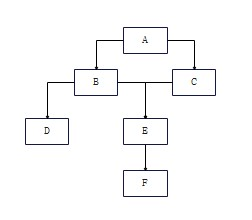
\includegraphics[width=0.5\linewidth]{CTG.jpg}
        \caption{控制流图}
        \label{fig:enter-label}
    \end{figure}
我们再以这张控制流图为例,来介绍确定语句线性序的算法。根据论文中的做法,我们从CTG的入口开始执行DFS,将每个结点都访问一次,在\textbf{退出}某一个节点时,输出该变量。那么,我们可以轻易得到这样的dfs顺序:$A\to B, B\to D, B\to E, E\to F, A\to C$,得到的输出结果是$D, F, E, B, C, A$。
然后,我们将其逆过来,即得到各基本块之间的线性序,即$A, C, B, E, F, D$。这就是基本块之间的线性序关系了。接下来,我们要做的无非是在基本块内对每一句语句进行标号了。这是平凡的。

\subsection{确定活跃区间}
这一部分请见活跃分析章节。我们只需要记录下每条语句处的活跃变量,根据每条语句的标号,对应地去更新这些变量的活跃变量即可。

\subsection{活跃区间排序}
\sout{不会吧不会吧,不会还有人优先级队列也不会用吧?真是杂鱼呢$\sim$}
这一部分的工作是非常平凡的。我们可以创造一个区间类,挑选一个心仪的容器,重载比较运算符,或者是用仿函数的方式确定区间类之间的大小关系进行排序即可。

\subsection{寄存器分配}
正如在该部分总述中的做法,不断对优先级队列执行出队操作,并检查是否有寄存器空闲:即该寄存器从来没有被指派过变量,或者指派给该寄存器之变量的活跃区间右端点小于当前分配变量的活跃区间之左端点。若有,则将当前变量分配给空闲的寄存器。如果没有,则将其溢出至栈上。

\subsection{总结}
不难发现,线性扫描算法是一种非常简洁,明确的寄存器分配算法。此外,如果向对线性扫描算法执行一定的优化,可以考虑进行区间拆分等操作,或是探索更合适的线性排序方法,或者可以考虑如何更好地对活跃区间排序等,于此不复赘述。

让我们动手吧!